\documentclass[11pt]{amsart}
\usepackage{amsmath,amssymb,amsthm}
\usepackage[margin=1in]{geometry}
\usepackage{microtype}
\usepackage{tikz}
\usetikzlibrary{arrows.meta,positioning}
\usepackage{hyperref}
\hypersetup{hidelinks}

\theoremstyle{plain}
\newtheorem{thm}{Theorem}[section]
\newtheorem{lem}[thm]{Lemma}
\newtheorem{prop}[thm]{Proposition}
\newtheorem{cor}[thm]{Corollary}
\newtheorem{conj}[thm]{Conjecture}
\theoremstyle{definition}
\newtheorem{defn}[thm]{Definition}
\newtheorem{rem}[thm]{Remark}

\DeclareMathOperator{\conv}{conv}
\DeclareMathOperator{\Pol}{Pol}
\DeclareMathOperator{\im}{im}
\DeclareMathOperator{\hgt}{height}
\DeclareMathOperator{\gen}{gen}
\DeclareMathOperator{\Ch}{Ch}
\newcommand{\B}{\{0,1\}}
\newcommand{\cube}{\square}
\newcommand{\atom}[1]{\langle #1 \rangle}

\title[A complexity dichotomy for order-convex monotone selection]
{A complexity dichotomy for order-convex monotone selection,\\
 with applications to Dedekind cubical sets}

\author{Ryota Shibusawa}
\address{Daiichi Institute of Technology, Japan}
\email{r-shibusawa@daiichi-koudai.ac.jp}

\subjclass[2020]{08A70, 68Q25; 08B05, 06D30, 55U35}
\keywords{constraint satisfaction, complexity dichotomy, bounded width,
  Taylor polymorphism, Siggers operation, order-convex set, monotone
  selection, distributive lattice, cubical set, Dedekind cube}

\begin{document}

\begin{abstract}
  We study the constraint language $L_m$ on the Boolean cube $\B^m$ whose
  relations are the order and all order-convex sets---the ambient
  language of \emph{monotone selection}, where one seeks a monotone map
  into prescribed order-convex fibres.  Its polymorphisms are the
  monotone, idempotent, order-convex-preserving operations, and they
  collapse sharply at $m=3$: for $m\le2$ the median is a majority
  polymorphism, so $L_m$ has bounded width and $\mathrm{CSP}(L_m)\in
  \mathrm P$; for every $m\ge3$ we prove that $\Pol(L_m)$ has neither a
  ternary weak near-unanimity nor a Siggers operation, so $L_m$ has
  \emph{unbounded width} and $\mathrm{CSP}(L_m)$ is
  $\mathrm{NP}$-complete.  Both obstructions are elementary hand proofs
  from small unsatisfiable cores that a machine locates (a twelve-cell
  and an eight-orbit contradiction on $\B^3$), propagated to all $m\ge3$
  by an order-convex restriction.

  The motivation and the application are homotopy-theoretic.  Monotone
  selection is the realizability engine of the Dedekind cubical site,
  whose type/test comparison the companion manuscript reduces to a chain-
  approximation master statement and two combinatorial cores.
  Median-closure of the fibres is the boundary for the \emph{canonical}
  median majority polymorphism---exactly the threshold the companion uses
  for strict width two---while the full ambient order-convex language
  undergoes its bounded-width and Taylor collapse at dimension three; we
  localize the two combinatorial cores onto the master statement:
  well-foundedness
  reduces to an $n$-coskeletality of atoms---which the strict-width-two
  mechanism above reduces, for median-fibre atoms, to a sharp
  pair-extension property, leaving that and the non-median-fibre residue
  conjectural---and the anchoring
  statement is shown \emph{equivalent} to chain approximation on the
  anchored subobjects of atoms.  Thus one homotopical core and two
  auxiliaries organize the Dedekind endgame, with the complexity
  dichotomy explaining why it pivots on median-closure.
\end{abstract}

\maketitle

\tableofcontents

\section{Introduction}

\subsection*{The phase diagram and its last open entry}
On each standard cube category the presheaves carry two canonical
homotopy theories: the cubical-type model structure of cubical type
theory, and Cisinski's test structure, which presents spaces; the type
structure presents spaces exactly when the two coincide.  The companion
manuscript~\cite{PaperW} completes this phase diagram except at the
\emph{Dedekind} site---the cube category with two connections---where it
reduces the comparison to a single approximation problem and localizes
the residue to two sharp combinatorial statements.  This paper studies
the structure of that residue.

\subsection*{The Dedekind cube and realizability}
The Dedekind cube category $\cube$ is the Lawvere theory of bounded
distributive lattices: a morphism $[k]\to[m]$ is a monotone map
$\B^k\to\B^m$.  A \emph{cell} of a presheaf is a monotone
$z\colon\B^m\to\B^n$; it generates the cyclic subpresheaf (\emph{atom})
$\atom{z}\subseteq\cube^n$ of all $z\circ g$, with image the marked
lattice $\im(z)\subseteq\B^n$.  Whether a cell $a$ is a face of $\atom z$
is a \emph{realizability} question---does $a$ factor as $z\circ g$ for a
monotone $g$?---which is, vertexwise, a monotone-selection constraint
problem: one variable $g(v)$ per vertex of the domain, with domain the
fibre $z^{-1}(a(v))$ and an order constraint along each edge.  This
constraint problem is the combinatorial engine of the whole endgame:
the coskeletal structure of atoms, the finiteness of the atom family,
and the chain-approximation statement all rest on it.

\subsection*{The master statement and the two cores (after~\cite{PaperW})}
Through Cisinski's regularity theory, a cosimplicial resolution by
cubical-simplex retracts, and a singular Quillen adjunction, \cite{PaperW}
proves the Dedekind comparison equivalent to a single
\emph{chain-approximation} statement: for every fibrant $X$ the inclusion
$\Ch(X)\hookrightarrow X$ of the intrinsic chain stratum is a type
equivalence.  The singular complex computes the test type of every
presheaf, so this is always a \emph{test} equivalence and only the
type-level upgrade remains; an audited assembly localizes that upgrade to
\begin{itemize}
\item[(a)] the subatom order of $\cube^n$ is well-founded;
\item[(b)] every subobject $W$ of a cyclic atom $A$, with $\Ch(A)
  \subseteq W\subseteq A$, is type-contractible (intrinsic
  chain-anchored asphericity).
\end{itemize}

\subsection*{Results of this paper}
The main theorem is the complexity dichotomy of
\emph{Part~\ref{part:cx}}: the order-convex language $L_m$ has bounded
width and is tractable for $m\le2$, and has unbounded width and is
$\mathrm{NP}$-complete for every $m\ge3$.  The full order-convex language
thus undergoes its bounded-width and Taylor collapse at dimension three,
while median-closure is exactly the condition that preserves the
\emph{canonical} median majority polymorphism for a fixed generator (Part
I is what makes the Dedekind engine pivot on median-closure; the two must
not be conflated, and \S\ref{sec:unified} keeps them apart).  The two
algebraic obstructions on $\B^3$---no ternary weak near-unanimity
operation, and no Siggers operation---are proved by hand from small
machine-located cores and lifted to all $m\ge3$ by an order-convex
restriction.  This is a self-contained result in the algebraic theory of
the CSP, entirely independent of the companion~\cite{PaperW}; the rest of
the paper is its cubical
application.  \emph{Part~\ref{part:a}} reduces the well-foundedness
statement (a) to the $n$-coskeletality of atoms---the naive height bound
on generation arity being false from $\cube^4$ on---which the
strict-width-two side of Theorem~\ref{thm:cx} reduces, for median-fibre
atoms, to a sharp pair-extension property (Proposition~\ref{prop:medred}),
leaving that and the non-median-fibre residue conjectural,
and \emph{Part~\ref{part:b}} shows the anchoring statement (b) is not an
independent obstruction at all: it is chain approximation itself,
evaluated on the anchored subobjects of atoms.  The logical shape of the
resulting endgame is drawn in Figure~\ref{fig:dep} and \S\ref{sec:unified};
Part~\ref{part:cx} is what makes it pivot on median-closure.

\begin{figure}[ht]
\centering
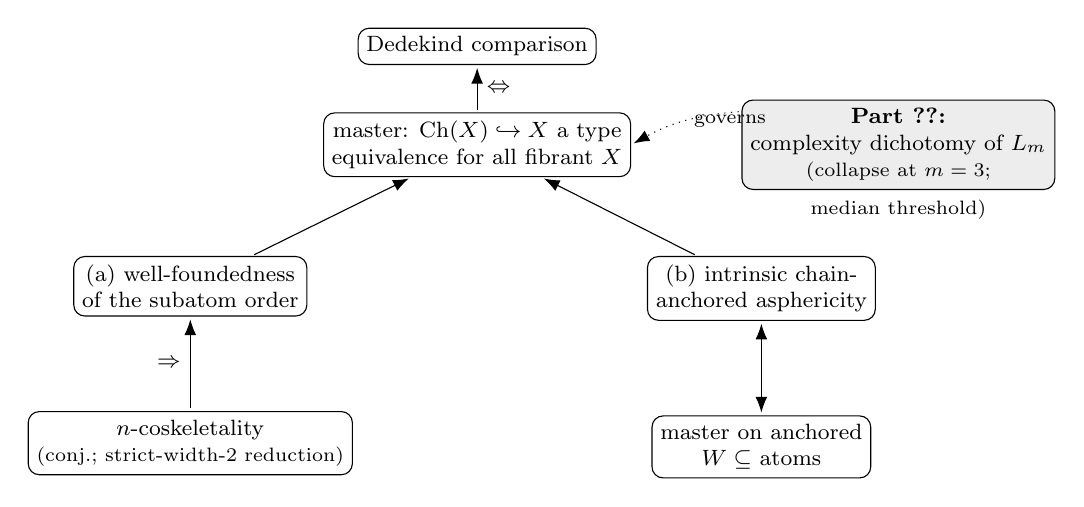
\begin{tikzpicture}[>={Latex[length=2mm]},node distance=6mm,
  every node/.style={font=\footnotesize},
  box/.style={draw,rounded corners,inner sep=3pt,align=center},
  proved/.style={box,fill=black!7},
  imp/.style={->,shorten >=1pt,shorten <=1pt}]
  \node[box] (ded) {Dedekind comparison};
  \node[box,below=of ded] (master) {master: $\Ch(X)\hookrightarrow X$ a type\\ equivalence for all fibrant $X$};
  \node[box,below left=10mm and 2mm of master] (a) {(a) well-foundedness\\ of the subatom order};
  \node[box,below right=10mm and 2mm of master] (b) {(b) intrinsic chain-\\anchored asphericity};
  \node[box,below=12mm of a] (bp) {$n$-coskeletality\\ \scriptsize (conj.; strict-width-2 reduction)};
  \node[box,below=12mm of b] (anch) {master on anchored\\ $W\subseteq$ atoms};
  \node[proved,right=14mm of master] (cx) {\textbf{Part~\ref{part:cx}:}\\ complexity dichotomy of $L_m$\\ \scriptsize (collapse at $m=3$;};
  \node[below=0pt of cx.south,font=\scriptsize] {median threshold)};
  \draw[imp] (master) -- node[right]{$\Leftrightarrow$} (ded);
  \draw[imp] (a) -- (master); \draw[imp] (b) -- (master);
  \draw[imp] (bp) -- node[left]{$\Rightarrow$} (a);
  \draw[imp,<->] (anch) -- (b);
  \draw[imp,dotted] (cx) to[bend right=12] node[right,pos=.5]{\scriptsize governs} (master.east);
\end{tikzpicture}
\caption{The shape of the Dedekind endgame.  The comparison is equivalent
to one master statement; its type-level upgrade was localized to (a) and
(b); (a) reduces to the $n$-coskeletality finiteness, and (b) is equivalent to the
master restricted to anchored subobjects.  Part~\ref{part:cx} governs the
whole: the order-convex language collapses (bounded width and tractability
lost) at $m=3$, and median-closure is the threshold that preserves the
canonical median polymorphism.}
\label{fig:dep}
\end{figure}

\subsection*{Related work}
Part~\ref{part:cx} lives in the algebraic theory of the constraint
satisfaction problem.  The tractable--intractable dividing line for a
fixed finite template is the Bulatov--Zhuk dichotomy \cite{Bulatov,Zhuk},
with tractability equivalent to a Taylor polymorphism, detected by the
single $4$-ary identity of Siggers \cite{Siggers,KMM}; the finer
bounded-width line is the Barto--Kozik theorem \cite{BartoKozik},
equivalent to weak near-unanimity terms of all but finitely many arities,
or to a linked ternary/quaternary WNU pair \cite{KKVW}.  Our
template $L_m$ carries \emph{all} order-convex unary relations, so its
polymorphisms are the monotone idempotent order-convex-preserving
operations; this places it near, but distinct from, the well-studied
\emph{conservative} languages (all unary relations present), whose
dichotomy is due to Bulatov and was reproved through binary structures by
Kazda and others \cite{BulatovCons,Kazda}.  The distinction is not
cosmetic: $L_m$ has only the \emph{order-convex} unary relations, a proper
subset---for instance $\{00,11\}\subseteq\B^2$ is not order-convex,
missing $01$ and $10$---so $\Pol(L_m)$ contains the polymorphism clone of
the \emph{conservative expansion} $(\B^m;\le,\text{all unary relations})$,
and $\mathrm{CSP}(L_m)$ is not an instance of the conservative dichotomy.
The containment is already \emph{strict} at $m=2$: $\Pol(L_2)$ contains
genuinely non-conservative operations, for instance the binary
\[
  f\bigl((x_1,x_2),(y_1,y_2)\bigr)=\bigl(y_1,\ y_2\vee(x_1\wedge x_2)\bigr)
\]
is monotone and idempotent, and lands in $\conv\{x,y\}$ (for $x\ne11$ it
equals $y$, and $f(11,y)\in[y,11]$), so it is a polymorphism of $L_2$ by
Lemma~\ref{lem:polchar}; yet $f(11,00)=01$ is neither argument.  Such
operations lie outside the conservative framework, and it is the
disappearance of the WNU/Taylor structure at $m=3$---rather than any
conservative-language obstruction---that Theorem~\ref{thm:cx} isolates.
Order-convex subsets of posets have also been studied from the
lattice-theoretic viewpoint---the lattice $\mathrm{Co}(P)$ of order-convex
sets and its sublattices~\cite{SemenovaWehrung}---whereas our question
concerns the clone simultaneously preserving the order and all order-convex
unary relations.
The novelty here is thus the specific
clone of order-convex-preserving operations on the Boolean cube, its sharp
collapse at $m=3$, and its role as the algebraic engine of a
homotopy-theoretic comparison---a bridge, to our knowledge new, between
the CSP dichotomy program and cubical model structures.  For the cubical
and homotopical background we depend on the companion~\cite{PaperW}; the
definitions and precise statements we use are recalled where needed.

\subsection*{On the use of machine computation}
The two algebraic obstructions on $\B^3$ are proved by hand, with the
machine only \emph{locating} a small unsatisfiable core: the
non-existence of a ternary weak near-unanimity operation reduces to a
twelve-cell contradiction, and the non-existence of a Siggers operation
to an eight-orbit one (both with an independent $\B^2$ satisfiability
check that returns the median resp.\ a Siggers operation).  The $n$-coskeletality of atoms is reduced, for the median-fibre class,
to a pair-extension property (Proposition~\ref{prop:medred}); it is
certified in the computed cases---median-fibre and residue alike---by an
exact interval-constraint factorization solver, not a bounded membership
search.  The
scripts are in the version-pinned artifact accompanying~\cite{PaperW}
(Zenodo, \texttt{doi:10.5281/zenodo.22247384}).  Every homotopical
statement is either proved or explicitly conjectural.

\part{The complexity dichotomy of order-convex monotone selection}
\label{part:cx}

% Part I: the complexity dichotomy of realizability (from the paperX note)

\section{The order-convex structure and its clone}

Realizability along $z$ has, as the cell $a$ varies, variable domains
the fibres $z^{-1}(a(v))$, which are \emph{order-convex}, and the single
binary constraint $\le$.  The natural template collecting all such
constraints is the following.

\begin{defn}
  A set $C\subseteq\B^m$ is \emph{order-convex} if $a,b\in C$ and $a\le
  c\le b$ imply $c\in C$.  Let $L_m$ be the relational structure on
  $\B^m$ with the order $\le$ and every order-convex subset as a unary
  relation, and $\Pol(L_m)$ its clone of polymorphisms.
\end{defn}

\begin{lem}\label{lem:polchar}
  $f\in\Pol(L_m)$ iff $f$ is monotone, idempotent, and
  \emph{order-convex-preserving}: $f(x_1,\dots,x_k)\in\conv\{x_1,\dots,
  x_k\}=\{c:\exists i,j\ x_i\le c\le x_j\}$.
\end{lem}
\begin{proof}
  Preserving $\le$ is monotonicity; singletons $\{a\}=[a,a]$ are
  order-convex, so preserving them is idempotence.  The convex hull is
  order-convex and contains the arguments, so preservation forces
  $f(\vec x)\in\conv\{\vec x\}$; conversely that condition makes $f$
  preserve every order-convex set containing all the $x_i$.
\end{proof}

An operation $w$ is a \emph{weak near-unanimity} (WNU) operation if it is
idempotent and $w(y,x,\dots,x)=w(x,y,x,\dots,x)=\cdots=w(x,\dots,x,y)$; we
write $m(x,y)=f(x,x,y)=f(x,y,x)=f(y,x,x)$ for a ternary one.  A finite
idempotent clone has \emph{bounded width} iff it has WNU polymorphisms of
all but finitely many arities, equivalently a ternary WNU $u$ and a
$4$-ary WNU $v$ with $u(x,x,y)=v(x,x,x,y)$ \cite{BartoKozik,KKVW}; it is
\emph{Taylor} (hence its CSP is in $\mathrm P$, by \cite{Bulatov,Zhuk})
iff it has a $4$-ary Siggers polymorphism $s(a,r,e,a)=s(r,a,r,e)$
\cite{Siggers,KMM}; otherwise the CSP is $\mathrm{NP}$-complete.  We
exclude a ternary WNU (Proposition~\ref{prop:base}) and a Siggers
operation (Proposition~\ref{prop:nosiggers}), so the conclusions below do
not depend on which equivalent formulation of bounded width one adopts.

\section{Reduction to the cube $\B^3$}

\begin{lem}[Order-convex restriction]\label{lem:restrict}
  Let $m\ge3$ and $T=\B^3\times\{0\}^{m-3}$, an interval hence
  order-convex.  Any $f\in\Pol(L_m)$ preserves $T$ and restricts to a
  polymorphism of $L_3$ on $T\cong\B^3$; the restriction inherits
  monotonicity, idempotence, and any WNU or Siggers identity of $f$.
\end{lem}
\begin{proof}
  $f$ preserves the order-convex $T$ (Lemma~\ref{lem:polchar}); an
  order-convex $C\subseteq T$ is order-convex in $\B^m$ (if $a\le c\le
  b$ with $a,b\in C\subseteq T$ then $c\in T$ by convexity of $T$, then
  $c\in C$), so $f|_T$ preserves it.  Identities restrict pointwise.
\end{proof}

Thus non-existence of a WNU or Siggers polymorphism on $\B^3$ propagates
to all $m\ge3$.

\section{The base case on $\B^3$}

\begin{prop}\label{prop:base}
  $\Pol(L_3)$ contains no ternary WNU operation.
\end{prop}
\begin{proof}[Proof (a twelve-cell contradiction)]
  Suppose $f$ is one.  For an antichain pair $\{x,y\}$,
  $\conv\{x,y\}=\{x,y\}$, so $m(x,y)\in\{x,y\}$; and $f(110,101,011)\in
  \{110,101,011\}$ (the coatoms are a $3$-antichain).  Consider the ten
  values
  \[\textstyle
  \begin{array}{llll}
  A=m(010,101), & B=m(100,011), & C=m(101,010), & D=m(101,011),\\
  E=m(101,110), & F=m(001,110), & G=f(110,101,011), & H=m(110,101),\\
  I=m(110,001), & J=m(110,011), & &
  \end{array}\]
  with domains the order-convex hulls
  ($A,C\in\{010,101\}$, $B\in\{011,100\}$, $D\in\{011,101\}$,
  $E,H\in\{101,110\}$, $F,I\in\{001,110\}$, $J\in\{011,110\}$,
  $G\in\{011,101,110\}$), and the monotonicities
  \[
    A\le G,H;\quad B\le D,G,J;\quad C\le D,E;\quad F\le E,G;\quad I\le H,J.
  \]
  As in Proposition~\ref{prop:nosiggers}, each is witnessed by two
  representatives comparable coordinatewise (the value is $f$ of any cell
  in its orbit, by the WNU identities):
  \begin{center}\small
  \renewcommand{\arraystretch}{1.05}\setlength{\tabcolsep}{4pt}
  \begin{tabular}{ccc@{\quad}ccc}
  \hline
  ineq. & rep.\ $\le$ & rep. & ineq. & rep.\ $\le$ & rep.\\
  \hline
  $A\le G$ & $(010,101,010)$ & $(110,101,011)$ & $C\le E$ & $(010,101,101)$ & $(110,101,101)$\\
  $A\le H$ & $(101,010,010)$ & $(101,110,110)$ & $F\le E$ & $(110,001,001)$ & $(110,101,101)$\\
  $B\le D$ & $(011,100,100)$ & $(011,101,101)$ & $F\le G$ & $(110,001,001)$ & $(110,101,011)$\\
  $B\le G$ & $(100,100,011)$ & $(110,101,011)$ & $I\le H$ & $(001,110,110)$ & $(101,110,110)$\\
  $B\le J$ & $(011,100,100)$ & $(011,110,110)$ & $I\le J$ & $(001,110,110)$ & $(011,110,110)$\\
  $C\le D$ & $(010,101,101)$ & $(011,101,101)$ & & &\\
  \hline
  \end{tabular}
  \end{center}
  If $B=011$ then $D=011$, $C=010$, $E=110$, $F=110$, $G=011$, and $F\le
  G$ fails ($110\not\le011$).  If $B=100$ then $D=101$, $C=101$,
  $E=101$, $F=001$, $G=101$, $A=101$, $H=101$, $I=001$, $J=110$, and
  $I\le J$ fails ($001\not\le110$).  Both cases are impossible.  (The
  twelve cells are a minimal unsatisfiable core located by machine; the
  deduction is by hand.)
\end{proof}

\begin{prop}\label{prop:nosiggers}
  $\Pol(L_3)$ contains no Siggers operation.
\end{prop}
\begin{proof}[Proof (an eight-variable contradiction)]
  Suppose $s\in\Pol(L_3)$ is a $4$-ary Siggers operation.  The Siggers
  identity $s(a,r,e,a)=s(r,a,r,e)$ groups the cells of $s$ into orbits;
  order-convex preservation puts each value in the convex hull of its
  arguments, and monotonicity relates comparable cells.  Consider the
  eight orbit-values
  \[
    P=s(110,001,001,110),\ Q=s(101,010,010,101),\ R=s(100,011,011,100),
  \]
  \[
    T=s(101,011,011,101),\ U=s(110,011,011,110),\ V=s(100,100,010,100),
  \]
  \[
    W=s(101,110,011,101),\ X=s(101,110,101,101),
  \]
  with domains the convex hulls
  \[
    P\in\{001,110\},\ Q\in\{010,101\},\ R\in\{011,100\},\ T\in\{011,101\},
  \]
  \[
    U\in\{011,110\},\ V\in\{010,100\},\ W\in\{011,101,110\},\ X\in\{101,110\},
  \]
  and the monotonicities
  \[
    P\le U,\ P\le W,\ P\le X,\ Q\le T,\ Q\le W,\ R\le T,\ R\le U,\ V\le W,\ V\le X.
  \]
  Each of these is witnessed by two orbit representatives that are
  comparable coordinatewise; since $s$ is constant on each orbit, the
  named value equals $s$ of the displayed representative, and
  monotonicity of $s$ gives the inequality.  The witnesses are:
  \begin{center}\small
  \renewcommand{\arraystretch}{1.05}
  \begin{tabular}{ccc}
  \hline
  inequality & representative $\le$ & representative\\
  \hline
  $P\le U$ & $s(110,001,001,110)$ & $s(110,011,011,110)$\\
  $P\le W$ & $s(110,001,110,001)$ & $s(110,101,110,011)$\\
  $P\le X$ & $s(110,001,001,110)$ & $s(110,101,101,110)$\\
  $Q\le T$ & $s(101,010,010,101)$ & $s(101,011,011,101)$\\
  $Q\le W$ & $s(101,010,010,101)$ & $s(101,110,011,101)$\\
  $R\le T$ & $s(100,011,011,100)$ & $s(101,011,011,101)$\\
  $R\le U$ & $s(100,011,011,100)$ & $s(110,011,011,110)$\\
  $V\le W$ & $s(100,100,010,100)$ & $s(101,110,011,101)$\\
  $V\le X$ & $s(100,100,010,100)$ & $s(110,101,110,101)$\\
  \hline
  \end{tabular}
  \end{center}
  (in each row the left argument tuple is $\le$ the right one in each of
  the four coordinates).  Split on $W$.  If $W=011$ then $P\le W$ forces $P=001$ and $V\le W$
  forces $V=010$; then $P\le X$ gives $X=101$, and $V\le X$ reads
  $010\le101$, false.  If $W=101$ then $P=001$, $Q=101$ (from $Q\le W$),
  $V=100$; $Q\le T$ gives $T=101$, $R\le T$ gives $R=100$, $R\le U$ gives
  $U=110$, and $P\le U$ reads $001\le110$, false.  If $W=110$ then
  $P=110$ and $Q=010$; $Q\le T$ gives $T=011$, $R\le T$ gives $R=011$,
  $R\le U$ gives $U=011$, and $P\le U$ reads $110\le011$, false.  All
  three cases are impossible.  (These eight orbits are a minimal
  unsatisfiable core located by machine; the deduction is by hand.  As a
  check the same search on $\B^2$ returns a Siggers operation.)
\end{proof}

\section{The dichotomy}

We record first the tractable side, for a single generator with
median-closed fibres.

\begin{prop}[median-closed fibres, after \cite{PaperW}]\label{prop:sw2}
  Let $z\colon\B^m\to\B^n$ be monotone with every fibre $z^{-1}(q)$
  closed under the ternary median $\mathrm{med}(x,y,z)=(x\wedge y)\vee
  (y\wedge z)\vee(z\wedge x)$.  Then the realizability problem along $z$
  carries the median as a majority polymorphism.  By the Baker--Pixley
  theorem \cite{BakerPixley} the solution relation of any instance is then
  determined by its binary projections; in the terminology of constraint
  satisfaction, a majority polymorphism yields \emph{strict width two}
  \cite{BartoKozik}: running the standard $(2,3)$-minimality
  (path-consistency) procedure on an instance produces a nonempty reduced
  instance exactly when the instance is solvable, decidable in polynomial
  time.  In particular the problem is in $\mathrm P$.
\end{prop}
\begin{proof}
  Applied coordinatewise the median preserves each fibre (they are
  median-closed) and the order $\{(x,y):x\le y\}$ (it is monotone), and
  satisfies the near-unanimity identities $\mathrm{med}(x,x,y)=
  \mathrm{med}(x,y,x)=\mathrm{med}(y,x,x)=x$; a ternary majority
  polymorphism gives strict width two \cite{BakerPixley,BartoKozik}.
\end{proof}

The contrast is total.

\begin{thm}\label{thm:cx}
  For $m\le2$ the order-convex language $L_m$ has bounded width (the
  median is a majority polymorphism) and $\mathrm{CSP}(L_m)\in\mathrm P$.
  For every $m\ge3$: $L_m$ has \emph{unbounded width}
  (Prop.~\ref{prop:base}, Lemma~\ref{lem:restrict}), $\Pol(L_m)$ is
  \emph{not Taylor} (Prop.~\ref{prop:nosiggers}, Lemma~\ref{lem:restrict}),
  and $\mathrm{CSP}(L_m)$ is $\mathrm{NP}$-complete.
\end{thm}
\begin{proof}
  The language $L_m$ contains every singleton $\{a\}=[a,a]$ (an
  order-convex set), so every retract of $L_m$ fixes each element:
  $L_m$ is a core and $\Pol(L_m)$ is idempotent.  The dichotomy
  \cite{Bulatov,Zhuk} in its idempotent formulation therefore applies
  directly, with no core reduction needed: $\mathrm{CSP}(L_m)$ is in
  $\mathrm P$ if $\Pol(L_m)$ is Taylor and $\mathrm{NP}$-complete
  otherwise.  For $m\le2$ the median is a Taylor (indeed majority)
  polymorphism: on $\B^{\le2}$ the coordinatewise median of any three
  vertices is one of the three ($\B^{\le1}$ is a chain, where this is
  clear; for $\B^2$, if the median differed from all three,
  each input would disagree with it in at least one of the two
  coordinates, so by the pigeonhole principle two inputs would disagree
  with it in the \emph{same} coordinate; but in that coordinate the median
  bit is the majority of the three input bits, which cannot differ from
  two of them---a contradiction.)  Being one of its arguments, the median
  preserves every unary relation, in particular every order-convex one,
  and it is monotone and idempotent---a majority polymorphism of $L_m$ by
  Lemma~\ref{lem:polchar}.  For $m\ge3$,
  by Lemma~\ref{lem:restrict} a ternary WNU
  or a Siggers operation of $\Pol(L_m)$ would restrict to one of
  $\Pol(L_3)$, which Propositions~\ref{prop:base} and~\ref{prop:nosiggers}
  exclude; so $\Pol(L_m)$ has no ternary WNU (unbounded width, by
  \cite{BartoKozik,KKVW}) and no Siggers operation (not Taylor, by
  \cite{Siggers,KMM}), and $\mathrm{CSP}(L_m)$ is $\mathrm{NP}$-complete.
\end{proof}

\begin{cor}[median-closure is the boundary for the canonical polymorphism]\label{cor:boundary}
  Median-closure of the fibres is the boundary for the \emph{canonical}
  coordinatewise median majority polymorphism of the realizability engine:
  \begin{enumerate}
  \item if a generator $z$ has median-closed fibres, realizability along
    $z$ has strict width two (Proposition~\ref{prop:sw2}) and is in
    $\mathrm P$;
  \item once a fibre is order-convex but not median-closed, the median is
    no longer a polymorphism, and the ambient order-convex constraint
    language $L_{m'}$ ($m'\ge3$)---the finite template with all
    order-convex relations---has unbounded width and is
    $\mathrm{NP}$-complete (Theorem~\ref{thm:cx}).
  \end{enumerate}
\end{cor}

Two cautions keep the statement honest.  First, part~(2) is a property of
the \emph{template} $L_{m'}$, not of any single generator: realizability
along a fixed $z$ uses only $z$'s own fibres and was polynomial in every
computed instance, so transferring the $\mathrm{NP}$-hardness to a uniform
cubical realizability problem would require a further reduction that we do
not carry out.  (The image $\im(z)$ need not be a sublattice---a monotone
$\B^3\to\B^3$ can have an $N_5$ image---so no distributivity is assumed.)  Second, the passage
from strict width two to a \emph{skeletally coskeletal} atom needs the
local-consistency step (three-dimensional realizability implies
$(2,3)$-consistency); Proposition~\ref{prop:medred} reduces it, for
median-fibre atoms, to a sharp pair-extension property that we verify
computationally but do not prove, so the coskeletal finiteness stays
conjectural (Part~\ref{part:a})---what is unconditional here is strict
width two itself.
What is unconditional is the algebraic dichotomy of
Theorem~\ref{thm:cx}, whose threshold is median-closure: Figure~\ref{fig:cube}
shows the elementary obstruction, the median of the three atoms escaping
their hull.

\begin{figure}[ht]
\centering
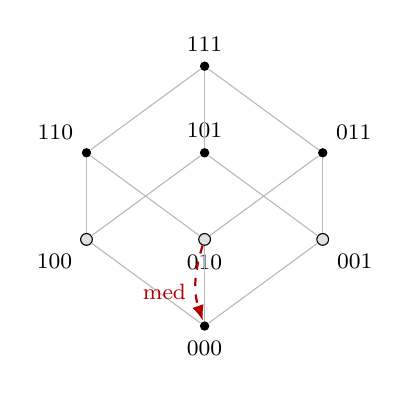
\begin{tikzpicture}[x=1.5cm,y=1.1cm,every node/.style={font=\footnotesize},
   dot/.style={circle,fill,inner sep=1.2pt},
   atom/.style={circle,draw,fill=black!12,inner sep=1.5pt}]
  \node[dot,label=below:$000$](b) at (0,0){};
  \node[atom,label=below left:$100$](a1) at (-1,1){};
  \node[atom,label=below:$010$](a2) at (0,1){};
  \node[atom,label=below right:$001$](a3) at (1,1){};
  \node[dot,label=above left:$110$](c1) at (-1,2){};
  \node[dot,label=above:$101$](c2) at (0,2){};
  \node[dot,label=above right:$011$](c3) at (1,2){};
  \node[dot,label=above:$111$](t) at (0,3){};
  \foreach \a/\c in {a1/c1,a1/c2,a2/c1,a2/c3,a3/c2,a3/c3}\draw[gray!55](\a)--(\c);
  \foreach \a in {a1,a2,a3}\draw[gray!55](b)--(\a);
  \foreach \c in {c1,c2,c3}\draw[gray!55](\c)--(t);
  \draw[-{Latex[length=2mm]},red!70!black,thick,dashed](a2) to[bend right=18] node[left,pos=.62]{$\mathrm{med}$}(b);
\end{tikzpicture}
\caption{The three atoms of $\B^3$ (shaded) form an antichain equal to
its own hull, but their median is the bottom $000$: no majority
operation compatible with the order-convex sets survives.}
\label{fig:cube}
\end{figure}


\bigskip
\begin{center}\large\bfseries Applications to the Dedekind cubical endgame\end{center}
\addcontentsline{toc}{part}{Applications to the Dedekind cubical endgame}
\nopagebreak

\part{Well-foundedness reduces to $n$-coskeletality}
\label{part:a}

% Part II: well-foundedness reduces to n-coskeletality (paperY note)

\section{The subatom order and its measure}

By Yoneda, $\atom{z'}\subseteq\atom z$ iff $z'=z\circ u$ for a monotone
$u$; a subatom is a substitution instance of its generator.  The
\emph{generation arity} $\gen(\atom z)$ is the least $k$ with a
generating cell $\B^k\to\B^n$, i.e.\ the least arity of a cell whose atom
equals $\atom z$.

\begin{lem}\label{lem:mono}
  If $\atom{z'}\subseteq\atom z$ then $\im(z')\subseteq\im(z)$, so
  $|\im|\in\mathbb N$ is non-increasing along the subatom order and
  bounded below by $1$.  Mutually cofinal atoms have equal image, so
  $\im$ and its order invariants ($\hgt$, $\operatorname{width}$) are
  invariants of the atom.
\end{lem}
\begin{proof}
  $z'=z\circ u$ gives $\im(z')=z(\im(u))\subseteq\im(z)$; if in addition
  $z=z'\circ u'$ then $\im(z)\subseteq\im(z')$, so $\im(z)=\im(z')$.
\end{proof}

The naive attempt to well-order the atoms by $\mu=|\im|$ fails at the
point noted in \cite{PaperW}: a proper inclusion need not decrease $\mu$,
since distinct atoms can share an image, and indeed a proper subatom can
share \emph{both} image and $|\im|$ with its parent.  What is true is
that the plateaus are controlled once the number of atoms per image is
finite.

\begin{prop}\label{prop:reduce}
  If for every finite bounded poset $L$ the atoms with image $L$ are
  finite in number, the subatom order is well-founded.
\end{prop}
\begin{proof}
  Along a descending chain $\atom{z_0}\supseteq\atom{z_1}\supseteq\cdots$
  the number $\mu=|\im|$ is non-increasing (Lemma~\ref{lem:mono}) and
  $\ge1$, hence eventually constant; from some index $N$ on
  $\im(z_{i+1})\subseteq\im(z_i)$ with equal cardinality, so
  $\im(z_{i+1})=\im(z_i)$, and all $z_i$ ($i\ge N$) share one image $L$.
  From $N$ on the chain lies in the finite class of atoms with image
  exactly $L$, and a strictly descending chain in a finite poset
  terminates.
\end{proof}

Thus a sufficient route to statement \textup{(a)} is finiteness of the
atom family, image by image.  The remaining sections locate that
finiteness.

\section{Generation arity is not bounded by height}

It is tempting to bound the generation arity by an order invariant of the
image, and the height $\hgt(\im z)$ is the natural candidate: it is
correct for every atom of $\cube^3$.  This bound is \emph{false} from
$\cube^4$ on, for a Sperner reason, and the failure is instructive
because it shows the finiteness of \textup{(a)} cannot come from a naive
arity bound.

Write $\operatorname{width}(L)$ for the largest antichain of $L$ and
\[
  \sigma(w)=\min\Bigl\{k:\tbinom{k}{\lfloor k/2\rfloor}\ge w\Bigr\}
\]
for the least arity whose cube $\B^k$ carries a $w$-element antichain
(Sperner).

\begin{prop}\label{prop:genwidth}
  For every atom, $\gen(\atom z)\ge\sigma\bigl(\operatorname{width}(\im
  z)\bigr)$.
\end{prop}
\begin{proof}
  Let $w:\B^k\to\B^n$ generate $\atom z$; by Lemma~\ref{lem:mono},
  $\im(w)=\im(z)$, so $\im(w)$ contains an antichain
  $a_1,\dots,a_{W}$ of size $W=\operatorname{width}(\im z)$.  Choose
  $v_i\in w^{-1}(a_i)$.  If $v_i\le v_j$ then $a_i=w(v_i)\le w(v_j)=a_j$,
  impossible for $i\ne j$; so $v_1,\dots,v_W$ is a $W$-antichain in
  $\B^k$.  Hence $\binom{k}{\lfloor k/2\rfloor}\ge W$, i.e.\
  $k\ge\sigma(W)$.
\end{proof}

\begin{prop}[failure of the height bound]\label{prop:nobound}
  For each $m\ge2$ let $P_m=\{\bot\}\cup A_m\cup\{\top\}\subseteq\B^{\sigma(m)}$
  with $A_m$ an $m$-element antichain.  Then $\hgt(P_m)=3$ while
  $\gen\ge\sigma(m)\to\infty$.  In particular the atom with image
  $P_4\subseteq\B^4$ has $\gen=4>3=\hgt$: the bound
  $\gen\le\hgt\circ\im$ fails on $\cube^4$, and generation arity is
  unbounded over images of bounded height.
\end{prop}
\begin{proof}
  $\hgt(P_m)=3$ (a longest chain is $\bot<a<\top$) and
  $\operatorname{width}(P_m)=m$, so $\gen\ge\sigma(m)$ by
  Proposition~\ref{prop:genwidth}.  For $m=4$, $\sigma(4)=4$; the cell
  $z\colon\B^4\to\B^4$ sending weight-$0$ to $\bot$, each weight-$1$
  vector to a distinct $a_i$, and everything of weight $\ge2$ to $\top$ is
  monotone with $\im(z)=P_4$, so $\gen\le4$, whence $\gen=4$.  The
  matching lower bound is exhaustively confirmed: all $160000$ monotone
  maps $\B^3\to\B^4$ have image of antichain-width $\le3$, so no cell of
  arity $\le3$ has a $4$-antichain image.

  For each $m\ge2$, pick an $m$-element antichain $a_1,\dots,a_m$ in the
  middle layer of $\B^{\sigma(m)}$ (possible as
  $\binom{\sigma(m)}{\lfloor\sigma(m)/2\rfloor}\ge m$), and define
  $z\colon\B^{\sigma(m)}\to\B^{\sigma(m)}$ by
  \[
    z(x)=\begin{cases}
    \bot & x<a_i\text{ for some }i,\\
    a_i & x=a_i,\\
    \top & \text{otherwise.}
    \end{cases}
  \]
  This is monotone---if $x\le y$ and $z(x)=a_i$ then $y=a_i$ or $y>a_i$,
  and $y>a_i$ lands in the ``otherwise'' case as no $a_j$ exceeds $a_i$,
  giving $z(y)=\top$; if $z(x)=\top$ then any $y\ge x$ is again neither
  below nor equal to an $a_j$, so $z(y)=\top$---and its image is exactly
  $P_m$.  Hence for every $m\ge2$ an atom with image $P_m$ exists, so
  generation arity is unbounded over images of height $3$.
\end{proof}

\begin{rem}[why $\cube^3$ hides the Sperner obstruction]
  For $n\le3$ every image $L\subseteq\B^n$ has
  $\operatorname{width}(L)\le3<4=\hgt(\B^3)$, and one checks on the $108$
  images of $\B^3\to\B^3$ that $\operatorname{width}(L)\le\hgt(L)$
  throughout; hence $\sigma(\operatorname{width}L)\le\hgt(L)$, so the
  Sperner lower bound of Proposition~\ref{prop:genwidth} cannot by itself
  violate the height bound below $\cube^4$.  The obstruction is exactly
  the first place antichains outgrow chains, $\binom{4}{2}=6>5$.
\end{rem}

\section{The correct reduction: \texorpdfstring{$n$}{n}-coskeletality}

The finiteness of \textup{(a)} is instead an $n$-\emph{coskeletality}
statement about the atom viewed as a sieve.  Recall the realizability
description of atoms: a monotone $h\colon\B^p\to\B^n$ lies in $\atom z$
iff it factors through $z$---at the level of vertices
$\im(h)\subseteq\im(z)$, and $h$ lifts monotonically along
$z\colon\B^m\twoheadrightarrow\im(z)$.

\begin{defn}
  The atom $\atom z\subseteq\cube^n$ is \emph{$n$-determined} if it is
  fixed by its cells of arity $\le n$: an $h$ of any arity lies in
  $\atom z$ as soon as this is forced by the arity-$\le n$ cells.  It is
  \emph{$d$-coskeletal} if a cell $h$ lies in $\atom z$ whenever every
  restriction $h\circ\varphi$ along a monotone $\varphi\colon\B^d\to\B^p$
  does (the forward direction is automatic; the content is the converse).
\end{defn}

\begin{rem}
  Testing exactly the arity-$d$ restrictions already sees all the
  arity-$k$ ones for $k\le d$: a cube projection
  $\pi\colon\B^d\twoheadrightarrow\B^k$ has a monotone section $s$, so a
  restriction $h\circ\psi$ ($\psi\colon\B^k\to\B^p$) equals
  $(h\circ\psi\circ\pi)\circ s$, a restriction of the arity-$d$ cell
  $h\circ\psi\circ\pi$; as $\atom z$ is a sieve, $h\circ\psi\circ\pi\in
  \atom z$ forces $h\circ\psi\in\atom z$.  So $d$-coskeletality is the
  restriction-determinacy of the sieve at level $d$; for these
  representable sieves it is the usual right-Kan-extension notion of
  $d$-coskeleton.
\end{rem}

\begin{rem}
  The restrictions run over \emph{all} monotone $\varphi\colon\B^d\to\B^p$,
  not merely the $2p$ facet inclusions.  This is essential: for the median
  atom below, testing only the eight facets of an arity-$4$ cell admits
  $104$ non-factoring cells that a non-facet (diagonal) restriction
  excludes, so facet-gluing alone would be false.
\end{rem}

\begin{prop}\label{prop:ndet}
  If every atom of $\cube^n$ is $n$-determined, there are finitely many
  atoms in $\cube^n$; hence, by Proposition~\ref{prop:reduce}, the
  subatom order is well-founded---statement \textup{(a)}.
\end{prop}
\begin{proof}
  An $n$-determined atom is fixed by its arity-$\le n$ data, a subset of
  the finite set $\prod_{k\le n}\mathrm{monotone}(\B^k,\B^n)$; so there
  are finitely many atoms, the subatom order is a finite poset, and a
  finite poset is well-founded (a fortiori Proposition~\ref{prop:reduce}
  applies).
\end{proof}

\begin{prop}\label{prop:cosk}
  $n$-coskeletality implies $n$-determinacy.
\end{prop}
\begin{proof}
  By $n$-coskeletality, $h\in\atom z$ iff every restriction $h\circ\varphi$
  along a monotone $\varphi\colon\B^n\to\B^p$ lies in $\atom z$; these are
  arity-$n$ cells, so membership of $h$ is a function of the arity-$\le n$
  part of the sieve.  Hence $\atom z$ is fixed by its arity-$\le n$ cells.
\end{proof}

Recall the local-consistency procedure used below.  Given a binary
constraint instance---variables with unary domains and binary constraints
on pairs---the standard $(2,3)$-\emph{minimality} procedure iteratively
deletes, from the constraint of each pair $(x,y)$, every admissible pair
$(a,b)$ for which some third variable admits no value $c$ with $(a,c)$ and
$(b,c)$ admissible, until a fixed point is reached; a pair \emph{survives}
if it is never deleted.  For a constraint language with a majority
polymorphism, the instance is solvable iff the resulting reduced instance
is nonempty (Proposition~\ref{prop:sw2}).  Nonemptiness of this reduced
instance is strictly stronger than the solvability of each three-variable
subproblem in isolation.

The median-closed case is where the tractable side of Part~\ref{part:cx}
enters, and it reduces $3$-coskeletality to a sharp local-consistency
question.

\begin{prop}[median-fibre reduction]\label{prop:medred}
  Let $z\colon\B^m\to\B^n$ be monotone with every fibre $z^{-1}(q)$ closed
  under the median.  Then the realizability problem along $z$ carries the
  median as a majority polymorphism, and:
  \begin{enumerate}
  \item (Proposition~\ref{prop:sw2}) it has \emph{strict width two}: an
    instance is solvable iff its $(2,3)$-minimal reduced instance is
    nonempty;
  \item the $3$-coskeletality hypothesis on a cell $h$---that
    $h\circ\varphi\in\atom z$ for every monotone $\varphi\colon\B^3\to\B^p$
    ---implies that every three-variable subproblem of the instance for
    $h$ is solvable.
  \end{enumerate}
  Consequently the pair-extension property below---that for these
  instances solvability of all three-variable subproblems forces the
  $(2,3)$-minimal reduced instance to be nonempty---is a \emph{sufficient}
  condition for $\atom z$ to be $3$-coskeletal.  \textup{(}The converse is
  not claimed:
  $3$-coskeletality constrains the eight-variable restrictions
  $h\circ\varphi$ directly, which triple-wise solvability need not.\textup{)}
\end{prop}
\begin{proof}
  Membership $a\in\atom z$ is the monotone-selection problem of
  Part~\ref{part:cx}: a monotone $g$ with $g(v)\in z^{-1}(a(v))$ for each
  vertex $v$ and $g(u)\le g(v)$ for $u\le v$.  The fibres are median-closed
  and the order $\{(x,y):x\le y\}$ is preserved by the coordinatewise
  median, so the median is a majority polymorphism, giving~(1) by
  Proposition~\ref{prop:sw2}.  For~(2), take any three vertices $u,v,w$ of
  the domain of $h$; their subposet has at most three elements, hence
  order-embeds into $\B^3$ by some $\iota$.  The partial monotone map
  $\iota(t)\mapsto t$ $(t\in\{u,v,w\})$ from a subposet of $\B^3$ into the
  complete lattice $\B^p$ extends to a monotone
  $\varphi\colon\B^3\to\B^p$, $\varphi(x)=\bigvee\{\,t\in\{u,v,w\}:
  \iota(t)\le x\,\}$ \textup{(}join taken in $\B^p$\textup{)}, with
  $\varphi(\iota(u))=u$, $\varphi(\iota(v))=v$, $\varphi(\iota(w))=w$.  By
  hypothesis $h\circ\varphi$ is solvable, and the restriction of a
  solution to $\iota(u),\iota(v),\iota(w)$ solves the subproblem on
  $\{u,v,w\}$.  The final clause combines~(1) with the definition of the
  $(2,3)$-minimal reduced instance.
\end{proof}

The remaining step is genuinely a step: a nonempty $(2,3)$-minimal reduced
instance asks that every \emph{surviving} pair assignment extend to every
third variable, which is stronger than the mere solvability of each triple.
We isolate it.

\begin{conj}[pair-extension for median fibres]\label{conj:pairext}
  For a median-fibre generator $z$ and a cell $h$ all of whose
  three-variable subproblems are solvable, the $(2,3)$-minimal reduced
  instance is nonempty \textup{(}equivalently, every surviving pair
  assignment extends to every third variable\textup{)}.  By
  Proposition~\ref{prop:medred} this would imply that every median-fibre
  atom is $3$-coskeletal.
\end{conj}

\begin{rem}[evidence]\label{rem:medev}
  The $3$-coskeletality \emph{conclusion} is machine-verified for the
  median atom of $\cube^3$: under the correct hypothesis \textup{(}all
  monotone $\varphi\colon\B^3\to\B^4$\textup{)} every boundary cell
  factors, with zero exceptions, whereas testing only the eight facets
  admits $104$ spurious cells that a diagonal restriction excludes.  (This
  confirms the conclusion of Conjecture~\ref{conj:pairext} for this atom,
  not the pair-extension property in isolation.)  Granting the conjecture,
  every
  atom with a median-fibre generator is $3$-coskeletal, hence
  $3$-determined; in $\cube^3$ all $174$ atoms generated at arity $\le3$
  carry a median-fibre generator, so all of them would be $3$-coskeletal,
  and the subatom order restricted to that class well-founded.
\end{rem}

The general conjecture below subsumes the median-fibre case; both are open.

\begin{conj}[$n$-coskeletality]\label{conj:cosk}
  Every atom of $\cube^n$ is $n$-coskeletal.
\end{conj}

\begin{rem}[Status]
  By Proposition~\ref{prop:medred} the median-fibre case is reduced to the
  pair-extension property (Conjecture~\ref{conj:pairext}); the harder
  residue is the class of atoms \emph{without} a median-fibre generator.
  Such atoms exist---they first appear at generation arity four, where a
  machine census finds $35$ of $150$ generators non-median-fibre---so the
  residue is nonempty and is exactly where the tractable mechanism of
  Part~\ref{part:cx} is unavailable (median-closure lost, the very
  threshold of Theorem~\ref{thm:cx}).  For both, the conjecture is
  supported by exhaustive and exact verification: $n=2$ is complete (all
  twelve atoms),
  and in $\cube^3$ the property is confirmed with an exact
  interval-constraint solver---not a bounded membership search---on
  several structurally distinct non-cube atoms, including a non-median,
  bare-variable one $\atom{(u\vee v,\,u\wedge w,\,u)}$ ($196$ of $196$
  boundary cells factor), and directly on non-median-fibre \emph{arity-four}
  generators, where membership is decided by the exact lift solver
  (a further such atom passes on all $2252$ boundary cells sampled).  No
  counterexample has ever appeared.  A proof for the residue is a
  local-to-global principle for monotone lifting with order-convex,
  non-median-closed fibres---precisely the hard regime of
  Theorem~\ref{thm:cx}---and would discharge \textup{(a)} outright.
\end{rem}

\begin{rem}[Compatibility with unbounded coskeletality]
  A non-median-fibre atom can have unbounded \emph{Kan} (right/coskeletal)
  dimension~\cite{PaperW} as its image grows; Conjecture~\ref{conj:cosk}
  is a \emph{skeletal} determinacy for each fixed $\cube^n$ and does not
  contradict it: granting Conjecture~\ref{conj:cosk}, for fixed $n$ the
  atoms are finite, and the unbounded Kan dimension appears only as
  $n\to\infty$.
\end{rem}


\part{Anchoring is chain approximation}
\label{part:b}

% Part III: anchoring is chain approximation (paperZ note)

\section{The intrinsic chain stratum of an anchored subobject}

The intrinsic chain stratum $\Ch(A)$ of an atom $A$ is the subpresheaf of
sorted cells and their chain instances---equivalently the image of
$\Ch_n$ under the sort action---which is functorial in maps of presheaves
\cite{PaperW}.  A subobject $W$ is \emph{anchored} if $\Ch(A)\subseteq
W\subseteq A$.

\begin{lem}\label{lem:chw}
  For an anchored subobject $W$, $\Ch(W)=\Ch(A)$.
\end{lem}
\begin{proof}
  Sortedness is a property of a cell itself, independent of the ambient
  object, so the sorted cells of $W$ are the sorted cells of $A$ lying in
  $W$; since $\Ch(A)\subseteq W$, these are all of $A$'s, and their chain
  instances again lie in $W$.  (Machine-checked on the median atom and
  others.)
\end{proof}

\section{Equivalence with chain approximation}

\begin{prop}\label{prop:bequiv}
  Let $A$ be a cyclic atom, so $\Ch(A)\hookrightarrow A$ is a type
  equivalence and $\Ch(A)$ is type-contractible \cite{PaperW}.  For an
  anchored $W$,
  \[
    W\text{ is type-contractible}\iff\Ch(W)\hookrightarrow W\text{ is a
    type equivalence.}
  \]
  Hence \textup{(b)} holds iff chain approximation holds on every
  anchored subobject of every cyclic atom---a sub-case of the master
  statement.
\end{prop}
\begin{proof}
  By Lemma~\ref{lem:chw}, $\Ch(W)=\Ch(A)$ is type-contractible.  If
  $\Ch(W)\hookrightarrow W$ is a type equivalence then $W\simeq\Ch(W)$ is
  contractible; conversely if $W$ is contractible then both $W$ and
  $\Ch(W)=\Ch(A)$ are contractible, so the inclusion is an equivalence.
\end{proof}

\begin{cor}
  For an anchored $W$, $\Ch(W)\hookrightarrow W$ is always a \emph{test}
  equivalence ($\Ch(W)=\Ch(A)$ is test-contractible and the singular
  complex computes the test type), so $W$ is test-contractible.  The
  content of \textup{(b)} is precisely the type-level upgrade---the same
  type-versus-test gap as the master statement, restricted to anchored
  subobjects.
\end{cor}

Thus (b) is not an independent homotopical obstruction: it is the master
chain-approximation statement itself, evaluated on the anchored
subobjects of atoms.  The lattice cone that contracts constant-free atoms
does not preserve the intrinsic stratum of the median atom, so a
non-cone, triangulation-level contraction is what a proof requires; every
computed anchored $W$ (sixteen atoms, median- and non-median-fibre alike)
is test-contractible, so the gap is a matter of proof mechanism, not a
counterexample.


\section{The unified endgame}
\label{sec:unified}

% Part IV: the unified picture

The three parts assemble into a single structure.  The Dedekind
comparison is, by \cite{PaperW}, equivalent to one homotopical
statement---chain approximation on all fibrant objects---and the two
combinatorial statements to which its type-level upgrade was localized
both feed that same core:
\[
  \small
  \boxed{\;
  \begin{array}{c}
  \textbf{master:}\ \ \Ch(X)\hookrightarrow X\ \text{a type equivalence
  for all fibrant }X\\
  \Longleftrightarrow\ \text{Dedekind comparison}\\[4pt]
  \text{(a) well-foundedness of the subatom order}\ \Longleftarrow\
  n\text{-coskeletality of atoms}\\[2pt]
  \text{(b) intrinsic chain-anchored asphericity}\ \Longleftrightarrow\
  \text{master on anchored }W\subseteq\text{atoms}
  \end{array}\;}
\]
Statement (a) is a \emph{finiteness}, orthogonal to the homotopy content:
it secures the well-founded induction that drives the assembly, and it
reduces to the $n$-coskeletality of atoms---a skeletal determinacy for
each fixed cube, untouched by the unbounded \emph{Kan} coskeletality of
non-median-fibre atoms.  The natural shortcut, a height bound on the
generation arity, is \emph{false} from $\cube^4$ on
(Proposition~\ref{prop:nobound}), which is exactly why the finiteness
must be carried by determinacy rather than by an elementary measure.
Statement (b) is not independent at all: it is the master statement
restricted to the anchored subobjects of atoms.  So the Dedekind endgame
has a single homotopical core and two auxiliaries---one a finiteness, one
an instance of the core.

Part~\ref{part:cx} explains \emph{why} the whole edifice pivots on
median-closure.  The realizability engine underlying atoms, coskeleta and
approximation is a monotone-selection constraint problem, and two
thresholds meet at the median mechanism.  For a \emph{fixed} generator,
median-closure of the fibres is exactly the condition that keeps the
canonical median a majority polymorphism, hence gives strict width two.
For the \emph{ambient} order-convex template, the bounded-width and Taylor
structure collapses at dimension three, so its $\mathrm{CSP}$ jumps to
unbounded width and $\mathrm{NP}$-completeness (Theorem~\ref{thm:cx}).  This is an algebraic dichotomy of the template,
sitting exactly at the threshold that governs the bounded-width mechanism
studied in \cite{PaperW}---the median majority polymorphism and its
strict-width/coskeletality program, whose passage from strict width two to
bounded coskeletality is itself left conjectural there; whether the
template dichotomy
transfers to a hardness statement about cubical realizability itself, or
whether (as our computations suggest) fixed-generator realizability stays
tractable, is a separate question we do not settle.  Even so, the
coincidence of the algebraic threshold with the homotopical one is the
structural reason the Dedekind site resists the elementary methods that
settle the other cube sites, and it locates what a resolution must
overcome: prove the $n$-coskeletality finiteness, and lift chain
approximation from test to type on the anchored subobjects of atoms---the
two faces, finite and homotopical, of the same median obstruction.

\begin{table}[ht]
\centering
\small
\renewcommand{\arraystretch}{1.2}
\begin{tabular}{l l p{0.34\textwidth}}
\hline
statement & status & reduces to\\
\hline
Dedekind comparison & open & the master statement \cite{PaperW}\\
master (chain approximation) & open & ---\\
(a) well-foundedness & open & $n$-coskeletality (Part~\ref{part:a}); median-fibre reduced to pair-extension\\
(b) anchored asphericity & open & master on anchored $W$ (Part~\ref{part:b})\\
median-closed realizability & \textbf{thm} & strict width two (Part~\ref{part:cx})\\
order-convex language $L_m$, $m\ge3$ & \textbf{thm} & unbounded width, $\mathrm{NP}$-complete (Part~\ref{part:cx})\\
fixed-generator realizability & \textbf{obs.} & $\mathrm P$ in all computed cases\\
\hline
\end{tabular}
\caption{The endgame at a glance: one homotopical core, two auxiliaries,
and the complexity dichotomy that pins the median-closure boundary.}
\end{table}


\section*{Declarations}

\noindent\textbf{Competing interests.}\quad The author declares that he has
no competing interests.

\noindent\textbf{Funding.}\quad No funding was received for this work.

\noindent\textbf{Ethical approval.}\quad Not applicable.

\noindent\textbf{Authors' contributions.}\quad R.\,Shibusawa is the sole
author and conceived, carried out, and wrote up the entire work.

\noindent\textbf{Availability of data and materials.}\quad The scripts
verifying the twelve-cell weak near-unanimity core and the eight-orbit
Siggers core, the Siggers SAT encodings, the Sperner-width refutation of
the height bound (Proposition~\ref{prop:nobound}), and the median-fibre and
non-median-fibre coskeletality checks are in the version-pinned artifact
accompanying~\cite{PaperW}
(Zenodo, \texttt{doi:10.5281/zenodo.22247384}).

\begin{thebibliography}{9}
\bibitem{PaperW}
R.~Shibusawa. Which cubical sites present spaces? Reflection subgroups,
connections, and the comparison of the type and test model structures.
Manuscript, 2026.
\bibitem{SemenovaWehrung}
M.~Semenova, F.~Wehrung. Sublattices of lattices of order-convex sets, I.
The main representation theorem. \emph{J.\ Algebra} \textbf{277} (2004),
825--860.
\bibitem{BakerPixley}
K.~A. Baker, A.~F. Pixley. Polynomial interpolation and the Chinese
remainder theorem for algebraic systems. \emph{Math.\ Z.} \textbf{143}
(1975), 165--174.
\bibitem{BartoKozik}
L.~Barto, M.~Kozik. Constraint satisfaction problems solvable by local
consistency methods. \emph{J.\ ACM} \textbf{61} (2014), Art.~3.
\bibitem{KKVW}
M.~Kozik, A.~Krokhin, M.~Valeriote, R.~Willard. Characterizations of
several Maltsev conditions. \emph{Algebra Universalis} \textbf{73}
(2015), 205--224.
\bibitem{Bulatov}
A.~A. Bulatov. A dichotomy theorem for nonuniform CSPs. \emph{58th
FOCS}, 2017, 319--330.
\bibitem{Zhuk}
D.~Zhuk. A proof of the CSP dichotomy conjecture. \emph{J.\ ACM}
\textbf{67} (2020), Art.~30.
\bibitem{Siggers}
M.~H. Siggers. A strong Mal'cev condition for locally finite varieties
omitting the unary type. \emph{Algebra Universalis} \textbf{64} (2010),
15--20.
\bibitem{KMM}
K.~A. Kearnes, P.~Markovi\'c, R.~McKenzie. Optimal strong Mal'cev
conditions for omitting type~$1$. \emph{Algebra Universalis} \textbf{72}
(2014), 91--100.
\bibitem{BulatovCons}
A.~A. Bulatov. Complexity of conservative constraint satisfaction
problems. \emph{ACM Trans.\ Comput.\ Log.} \textbf{12} (2011), Art.~24.
\bibitem{Kazda}
A.~Kazda. CSP for binary conservative relational structures.
\emph{Algebra Universalis} \textbf{75} (2016), 75--84.
\end{thebibliography}

\end{document}
